\documentclass [a4paper] {report}
\usepackage{amsmath,amssymb,amsthm, bbm, graphicx,listings,braket,subfig,titlesec,cleveref,lipsum,mcode,xcolor-patch, textcomp,float,booktabs,siunitx, listings}
\usepackage[authoryear]{natbib}
\usepackage[section]{placeins}
\usepackage[margin=2.2cm]{geometry}
\titleformat{\chapter}{\normalfont\huge}{\thechapter.}{20pt}{\huge \bf}

\DeclareMathOperator*{\argmin}{arg\,min}
\DeclareMathOperator*{\argmax}{arg\,max}
\newcommand{\norm}[1]{\left\lVert #1 \right\rVert}

\begin{document}
	
	\begin{titlepage}
		\begin{center}
			
			\textsc{\LARGE IN4320 Machine Learning}\\[1.25cm]
			
			\rule{\linewidth}{0.5mm}\\[1.0cm]
			{\huge \bfseries Exercises: Covariate Shift }\\[0.6cm]
			\rule{\linewidth}{0.5mm}\\[1.5cm]
			
			\begin{minipage}{0.4\textwidth}
				\begin{flushleft} \large	
					\emph{Author:}\\
					\textsc{Milan Niestijl, 4311728}
				\end{flushleft}
			\end{minipage}
			
			\vfill
			{\large \today}
		\end{center}
	\end{titlepage}
	
	\section*{1. Questions}
	
	\subsection*{1.1}
	Suppose the problem is to asses the risk of a hart attack within three years, $\mathbf{y}$, given the recent past of drug abuse, $\mathbf{x}$. Suppose some algorithm is trained on data obtained in a certain country, say, the Netherlands, but the task becomes to make a prediction in another country in which drug abuse is much less common, for instance due to much more strict laws. In this case it is reasonable to assume that the posterior probability $\mathbb{P}(\mathbf{y}|\mathbf{x})$ has not changed, as the bodies of the people living in both countries react approximately the same to drugs. However, the marginal probability $\mathbb{P}(\mathbf{x})$ has changed. Therefore, this is an example of a covariate shift setting with the Netherlands being the source domain and the other country being the target domain. The question now becomes how the algorithm can be adapted to the new situation using the training data from the source domain and samples from the joint distribution in the target domain.
	
	\subsection*{1.2}
	The ratio might decay to zero very quickly, causing most of the samples in the source domain to receive (near) zero weight, which effectively reduces the number of training samples by a potentially drastic amount. This results in poor performance of the classifier.
	
	\subsection*{1.3}
	Let $\mathcal{S}$ and $\tau$ random variables corresponding to the source and target domain, respectively. Denote their probability density function by $p_{\mathcal{S}}(x)$ and $p_{\tau}(x)$. \\
	
	The sample average of the weights is constrained to be close to one since it approximates the integral of $p_{\tau}(x)$ over the sample space $\Omega$, which has to equal one by the definition of a probability space:
	\begin{align*}
		1 &= \int_{\Omega} p_{\tau}(x)dx\\
		&= \int_{\Omega} {p_{\tau}(x) \over p_{\mathcal{S}}(x)}p_{\mathcal{S}}(x)dx\\
		&= \int_{\Omega} w(x)p_{\mathcal{S}}(x)dx\\
		&= \mathbb{E}(w(\mathcal{S}))\\
		&\approx {1\over n} \sum_{i=1}^{N}  w(x_{i})
	\end{align*}
	
	\newpage
	\section*{2. Code Assignment}
	The Kernel Mean Matching algorithm was implemented using Matlab, with regularization parameter $\lambda=2$ and constraint loosening parameter $\epsilon=0.01$. The code is provided at the end of the report. The resulting weighted and unweighted least-squares classifiers are shown in figures \ref{plot} and \ref{hist}. 
	
	\begin{figure}[H]
		\begin{center}
			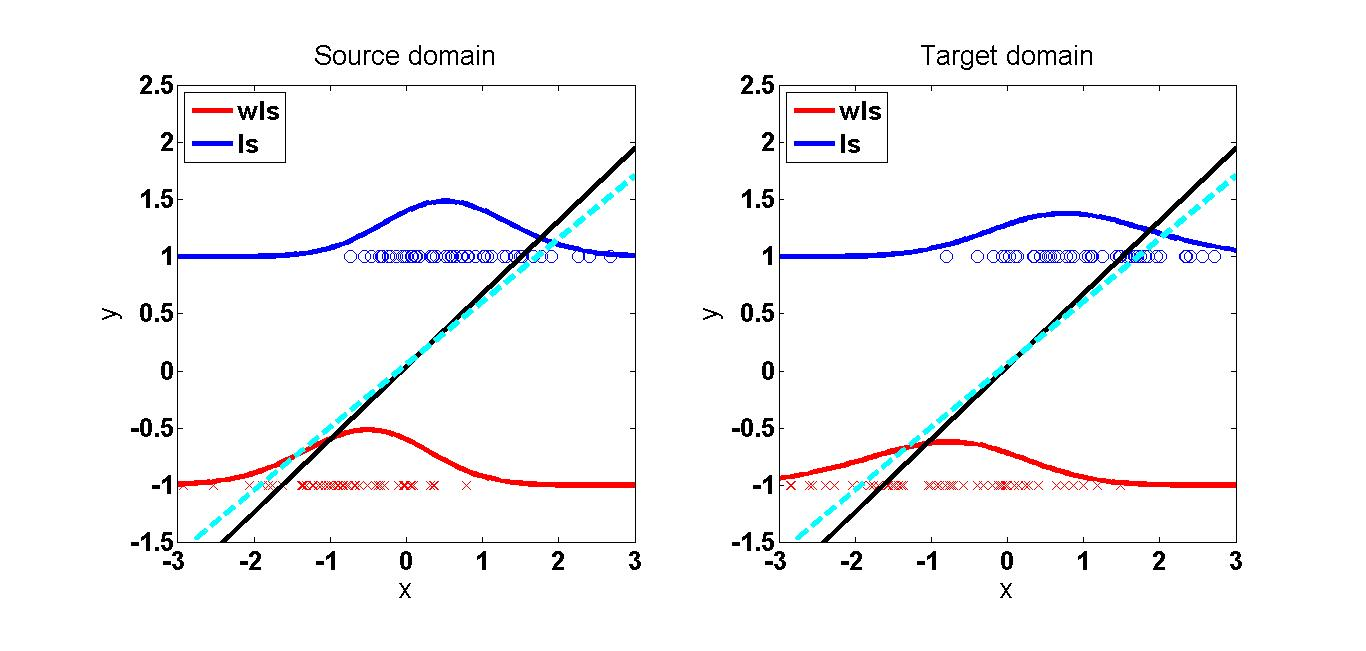
\includegraphics[scale=0.35]{Images/Plot_lambda2eps0_01.jpg}
			\caption{Plot of both the unweighted $(ls)$ and the weighted $(wls)$ least-squares classifier on a randomly generated dataset.}
			\label{plot}
		\end{center}
	\end{figure}
	
	\begin{figure}[H]
		\begin{center}
			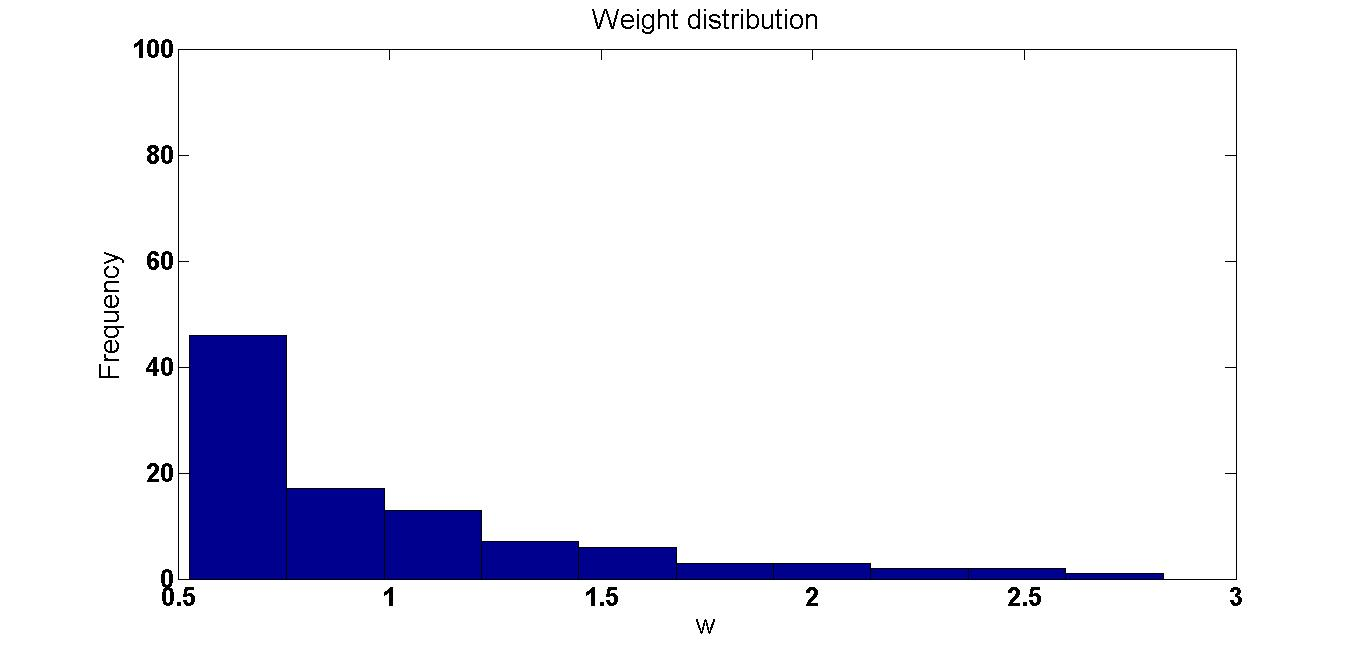
\includegraphics[scale=0.3]{Images/Hist_lambda2eps0_01.jpg}
			\caption{Histogram of the estimated sample weights using kernel mean matching.}
			\label{hist}
		\end{center}
	\end{figure}
	
	\newpage
	\section*{Code}
	
	Note that the code differs slightly from the code on Blackboard, since an older version of Matlab was used (2013a).
	
	\begin{lstlisting}
function [w] = kmm(X,Z)
% Estimate weights using Kernel Mean Matching
% Paper: Huang, Smola, Gretton, Borgwardt, Schoelkopf (2006)
% Correcting Sample Selection Bias by Unlabeled Data
%
% Input:
%       X       = source data (n x 1)
%       Z       = target data (m x 1)
% Output:
%       w       = weights (n x 1)
%
% Author: Wouter Kouw
% Last update: 28-03-2017

%% Initialization
% Sizes
n = size(X,1);
m = size(Z,1);

% Optimization options
options = optimoptions('quadprog', 'Display', 'final', ...
'Algorithm', 'interior-point-convex',...
'TolX', 1e-5, ...
'maxIter', 1e2);

% |mean(w)-1|<eps
eps = 0.01; 

% regularization
lambda = 2;

% RBF kernel
K = @(x1,x2) exp(-1/2*norm(x1-x2)^2);

% Create kernel matrix Kmat and vector k
Kmat = zeros(n,n);
k = zeros(m,1);
for i=1:n
	for j=1:m
	Kmat(i,j) = 2/(n^2) * K(X(i,:),X(j,:));
	end
	k(i) = -2/(m*n) * sum(arrayfun(@(j) K(X(i,:),Z(j,:)),1:m));
end
Kmat = Kmat + 2/(n^2).*lambda.*eye(n);

%% Solve quadratic program minimize w.r.t. w:
%       1/n^2 w'Kw - 2/(m*n) w'k 
%       s. t. |mean(w)-1| = epsilon and w >= 0

% define constraints
A = 1./n .* [ones(1,n); -ones(1,n);zeros(n-2,n)];
b = [1+eps; eps-1; zeros(n-2,1)]; 
lb = zeros(n,1);
ub = n*ones(n,1);
x0 = ones(n,1);

% solve program
w = quadprog(Kmat,k,A,b,[],[],lb,ub,x0,options);
end
	\end{lstlisting}

\end{document}